% !TeX root = ../main.tex
\documentclass[./../main.tex]{subfiles}

\begin{document}

Những kẻ tấn công bằng nhiều cách có thể cài đặt các phần mềm độc hại trên máy nạn nhân để có được quyền truy cập, thực hiện các hành vi xâm phạm dữ liệu cá nhân hay dữ liệu nhạy cảm, phá hoại hệ thống hoặc sử dụng vào những mục đích xấu khác. Người dùng thường có thể dễ dàng nhận ra mối đe dọa từ những tệp thực thi, ngoài ra nhận thức về mối nguy hiểm từ các tài liệu Microsoft Office cũng ngày càng tăng cao. Tuy nhiên, bỏ qua sự phức tạp về định dạng cấu trúc tệp PDF, người dùng có xu hướng coi các tệp PDF là tài liệu vô hại.

Hiện nay, lợi dụng các lỗ hổng bảo mật, các trình đọc tài liệu PDF đang là mục tiêu của các kẻ tấn công mạng. Điển hình với trình đọc PDF Acrobat Reader, từ năm 1999 tới nay, đã có tới 298 lỗ hổng được phát hiện theo thống kê của CVE Details.
\begin{figure}[ht!]
	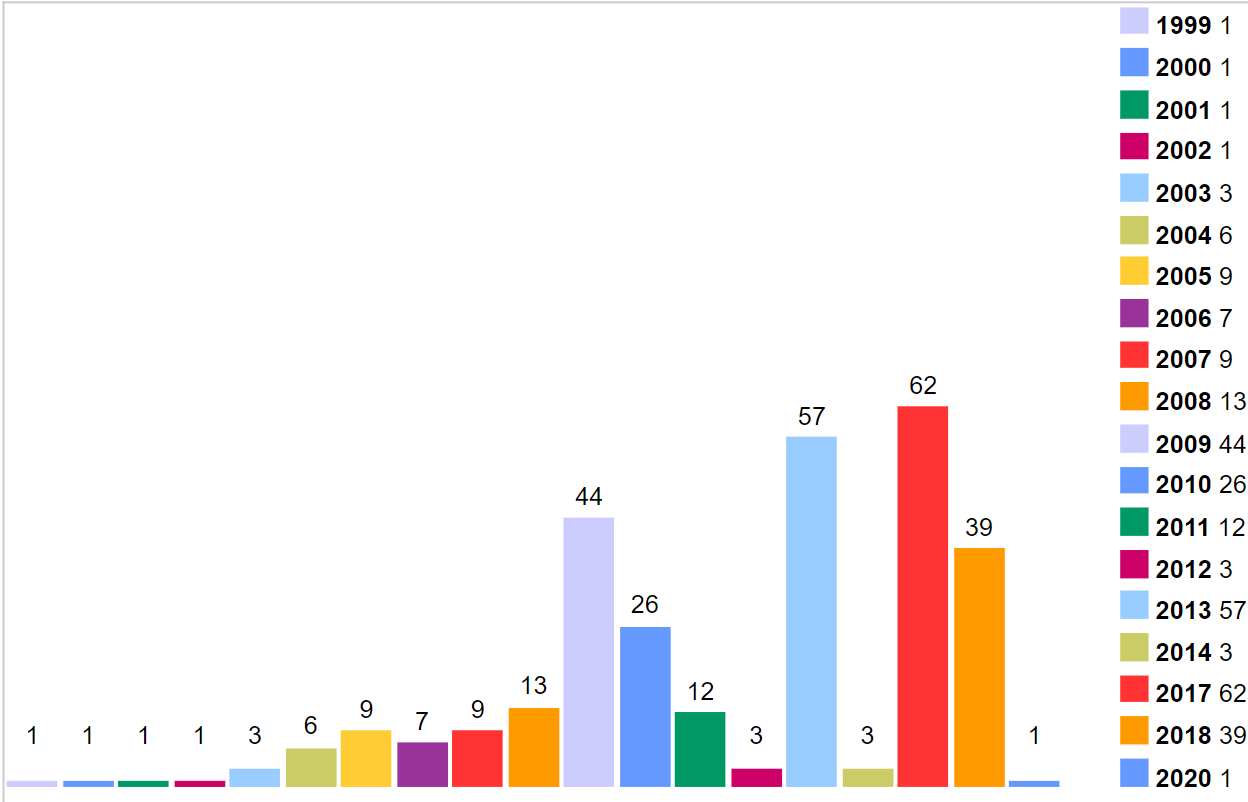
\includegraphics[width=\linewidth]{./images/img2_acrobatcve.png}
	\caption{Biểu đồ các lỗ hổng của trình đọc PDF Acrobat Reader theo các năm}
	\label{fig:component}
\end{figure}


Trong khóa luận này, em sẽ trình bày một số phương pháp để phát hiện các tệp PDF độc hại, trong đó các đặc trưng được trích xuất từ tài liệu PDF sẽ được sử dụng để xây dựng bộ phân loại học máy tự động phát hiện tài liệu PDF độc hại, thông qua các chương sau:
\begin{description}
	\item [Chương 1] Kiến thức nền tảng về định dạng tài liệu PDF, kỹ thuật sử dụng trong tài liệu PDF độc hại, từ đó đưa ra phương pháp phát hiện phần mềm độc hại.
	\item [Chương 2] Đi sâu vào các phương hướng trích xuất đặc trưng hiện nay, gồm các đặc trưng dựa trên từ khóa, cấu trúc tài liệu và cuối cùng là dựa trên mã nhúng
	\item [Chương 3] Thực hiện thí nghiệm trích xuất đặc trưng được đề xuất ở chương 2, từ đó xây dựng bộ phân loại và đánh giá kết hợp các đặc trưng khác nhau
	\item [Chương 4] Thực hiện thí nghiệm xây dựng mô hình học máy không gán nhãn độc sai. Chứng minh qua lập luận và kết quả thí nghiệm trên các tập dữ liệu khác nhau.
	\item [Kết luận] Đánh giá kết quả đạt được, hạn chế và khó khăn gặp phải, và cuối cùng đề xuất các hướng mới để phát triển đề tài.
\end{description}
\end{document}